\subsection{Data samples and event selection}

This analysis is based on PbPb and pp data collected with the CMS detector at 2.76 TeV and 5.02 TeV during Run 1 and Run 2 of the CERN LHC.  Studies at 2.76 TeV use 166 $\mu {\rm b}^{-1}$ of PbPb data collected in 2011, and 5.3 pb$^{-1}$ of pp data collected in 2013.  Studies at 5.02 TeV use 404 $\mu {\rm b}^{-1}$ of PbPb data and 25 pb$^{-1}$ of pp data, both collected in 2015.  Online collision selection was performed using the CMS HLT described in Sec.~\ref{sec:HLT} to obtain a minimum bias sample of PbPb collision events, and to obtain samples of PbPb and pp data with the requirement that events contain at least one high-$p_{\rm T}$ jet (with $p_{\rm T} > 80$~GeV for pp data and 2.76 TeV PbPb data, $p_{\rm T} > 100$~GeV for 5.02 TeV PbPb data).  These jet triggers are fully efficient for offline-reconstructed jets with $p_{\rm T} > 120$~GeV.  Total numbers of selected events are summarized in Table~\ref{table:evt_sel}.

\begin{table}[h!]
\begin{center} 
\caption{Summary of data samples and number of selected events}
\label{table:evt_sel} 
\begin{tabular}{|c|c|c|c|}
\hline
\hline
Dataset & Number of selected events  \\
\hline
\hline
2.76 TeV PbPb MinimumBias & 1.01 M \\
2.76 TeV PbPb Jet-triggered ($p_{\rm T} > 80$~GeV) & 1.25 M \\
2.76 TeV pp Jet-triggered ($p_{\rm T} > 80$~GeV) & 1.27 M \\
\hline
\hline
5.02 TeV PbPb MinimumBias & 764 k \\
5.02 TeV PbPb Jet-triggered ($p_{\rm T} > 100$~GeV) & 3.35 M \\
5.02 TeV pp Jet-triggered ($p_{\rm T} > 80$~GeV) & 2.66 M\\
\hline
\hline
\end{tabular}
\end{center} 
\end{table} 

A number of quality cuts are applied, as is standard for CMS analyses to remove detector noise backgrounds, ultra-peripheral collisions, beam gas, and events with exceptionally large pixel occupancy. These selection criteria have shown to have negligible impact on dijet analyses~\cite{Chatrchyan:2012gt,Chatrchyan:2012gw}, and are as follows in PbPb and pp collisions: 
\begin{itemize}
\item Vertex-z position within 15 cm of the center of the detector ($|\rm v_{z}| < 15$)
\item Primary vertex filter -- a requirement that events include a reconstructed primary vertex filter with at least two tracks, requiring the presence of inelastic hadronic scattering and removing beam-gas events and ultra-peripheral collisions
\item Beam-scraping filter -- a requirement of pixel clusters compatible with the primary vertex.  In pp, this requires that if there are more than 10 tracks, at least 25\% of tracks must be highPurity (see Sec.~\ref{sec:Tracks})
\item HB/HE noise filter -- a filter to exclude events exhibiting uncharacteristic calorimeter noise~\cite{Chatrchyan:2009hy}
\item PbPb data only:  HF coincidence filter -- at least 3~GeV recorded in at least each of at least three hadronic forward calorimeter towers on each side of the interaction point
\end{itemize}

\noindent These cleaning cuts are applied to both minimum bias and jet-triggered data samples.  Additional event selection will later be applied to obtain samples of high-$p_{\rm T}$ jets and dijet events, as discussed in Sec.~\ref{sec:jet_sel} below. 



\subsection{Collision centrality determination and classes}
\label{sec:centrality}

The variable centrality is used to parameterize the degree of overlap of the colliding nuclei.  In CMS, centrality is determined using total transverse energy ($E_{\rm T}$) in the HF calorimeter towers, in the region $4.0 < |\eta| < 5.2$.  The distribution of total $E_{\rm T}$ in all events is used to divide the total minimum bias event sample into centrality bins, each containing 0.5\% of the total events.  The resulting centrality distribution is flat in minimum bias data by construction.  In jet-triggered, data, however, requiring the presence of a high-$p_{\rm T}$ jet results in a larger fraction of more central collisions (in which hard-scatterings are more likely).  The collisions defined as ``most central'' (centrality = 0\%) are those with the greatest $E_{\rm T}$, corresponding to collisions in which the nuclei collided head-on.  In contrast, the collisions defined as ``least central'' or ``most peripheral'' (centrality = 100\%) are those in which the nuclei barely overlapped at all.  To observe how jet modifications evolve with changing centrality, this analysis considers four centrality classes:  0-10\% (most central), 10-30\%, 30-50\%, and 50-100\%.

\subsection{Monte Carlo simulation}

Monte Carlo (MC) simulation is used in this analysis to evaluate and correct for jet reconstruction performance and tracking efficiency for both pp and PbPb data.  Simulation of pp data and of the hard processes in PbPb data are performed using the {\sc pythia} (version 6, tune Z2~\cite{bib_pythia}) event generator. In order to have reasonable event samples in all jet $p_{\rm T}$ ranges, different samples are produced with various cut-off values of $\hat{p_{\rm T}}$, which are then combined using their respective cross-sections as weights.  To simulate CMS detector output for MC events, {\sc geant}4 detector simulation is used~\cite{bib_geant}.  Jet and track reconstruction performance and efficiency for pp data is evaluated by comparing observables in {\sc pythia} samples as generated to the same observables after they have been passed through the detector simulation and the same reconstruction procedures applied to pp data.  For the relevant jet kinematics observables relevant to this analysis, {\sc pythia} reasonably reproduces pp data.  

For PbPb data, the underlying event is simulated using {\sc hydjet} (Drum5 tune)~\cite{Lokhtin:2005px}, which combines hydrodynamics with ``mini-jets''  produced with quenched pythia input.  Hard processes are generated using {\sc pythia}, and are directly embedded in this {\sc hydjet} sample (refered to as {\sc pythia+hydjet} simulation), with no medium quenching effects applied to the embedded jets.  This {\sc pythia+hydjet} sample is used to evaluate the reconstruction effects of the presence of the QGP medium, $other$ than the jet-medium interactions that are our objects of study.  As for {\sc pythia} simulation of pp data, comparing {\sc pythia+hydjet} samples that have been passed through the detector and reconstructed chain to the generated Monte Carlo allows for the evaluation of jet and track reconstruction performance.  


\subsubsection{Monte Carlo centrality and vertex-z reweighting}

Simulated {\sc pythia+hydjet} samples are generated minimum bias, and therefore must be reweighted to match the bias toward more central events induced by requiring the presence of a high-$p_{\rm T}$ jets discussed in Sec.~\ref{sec:centrality}.  Reweighting factors are calculated for each 0.5\%-wide centrality bin, and applied to the {\sc pythia+hydjet} sample overall to match the PbPb centrality distribution.  Similarly, another reweighting procedure is performed to match the distributions of the position of the primary interaction along the beam direction in MC and data for both pp and PbPb collisions.  Figures~\ref{fig:HydCent_Reweighting}-\ref{fig:PythiaVz_Reweighting} illustrate the necessity and effects of these reweighting procedures.  


\begin{figure}[ht]
\begin {center}
  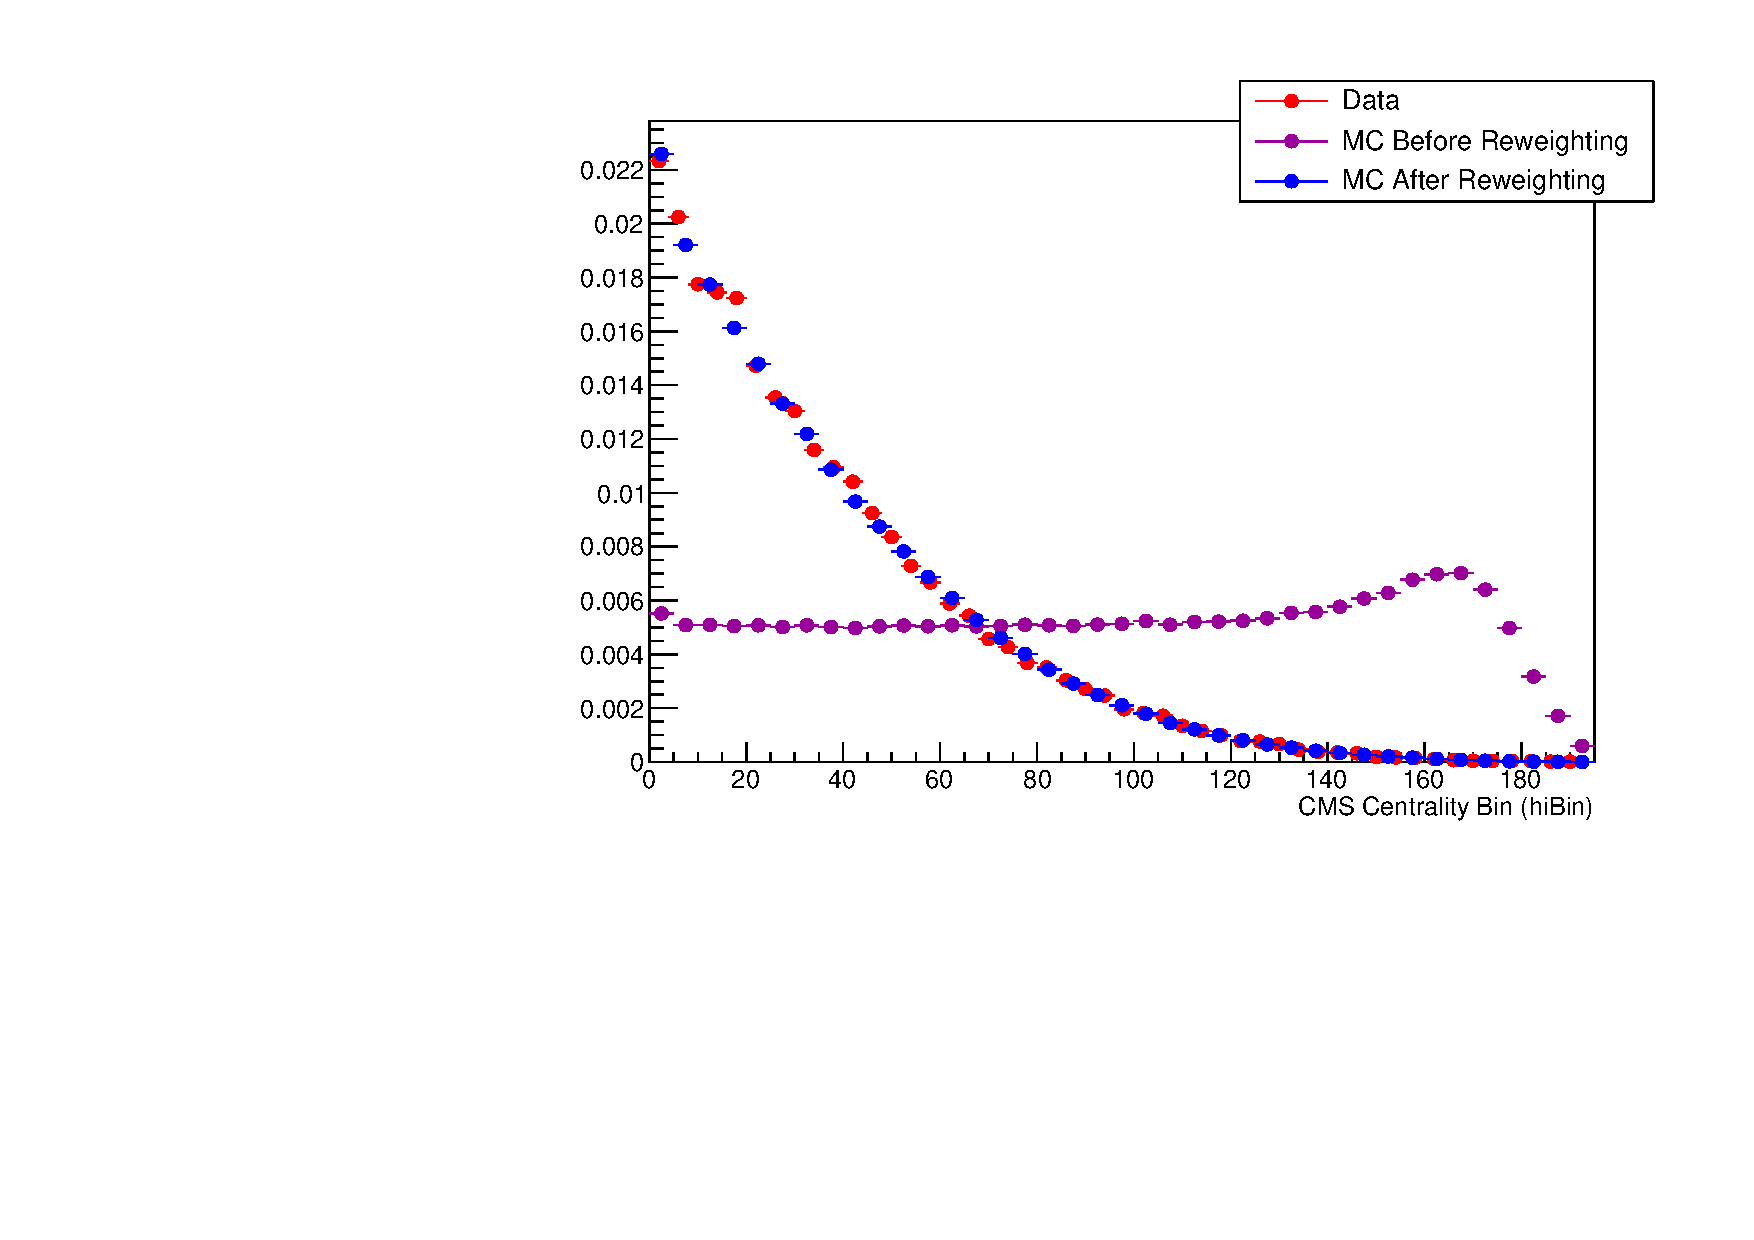
\includegraphics[width=0.58\linewidth]{figures/Samples/HydjetCentralityReweighting.pdf}
  \caption{
    Centrality distribution for {\sc pythia+hydjet} reweighted to match centrality distribution of PbPb data.
  }
\label{fig:HydCent_Reweighting}
\end{center}
\end{figure}



\begin{figure}[ht]
\begin {center}
  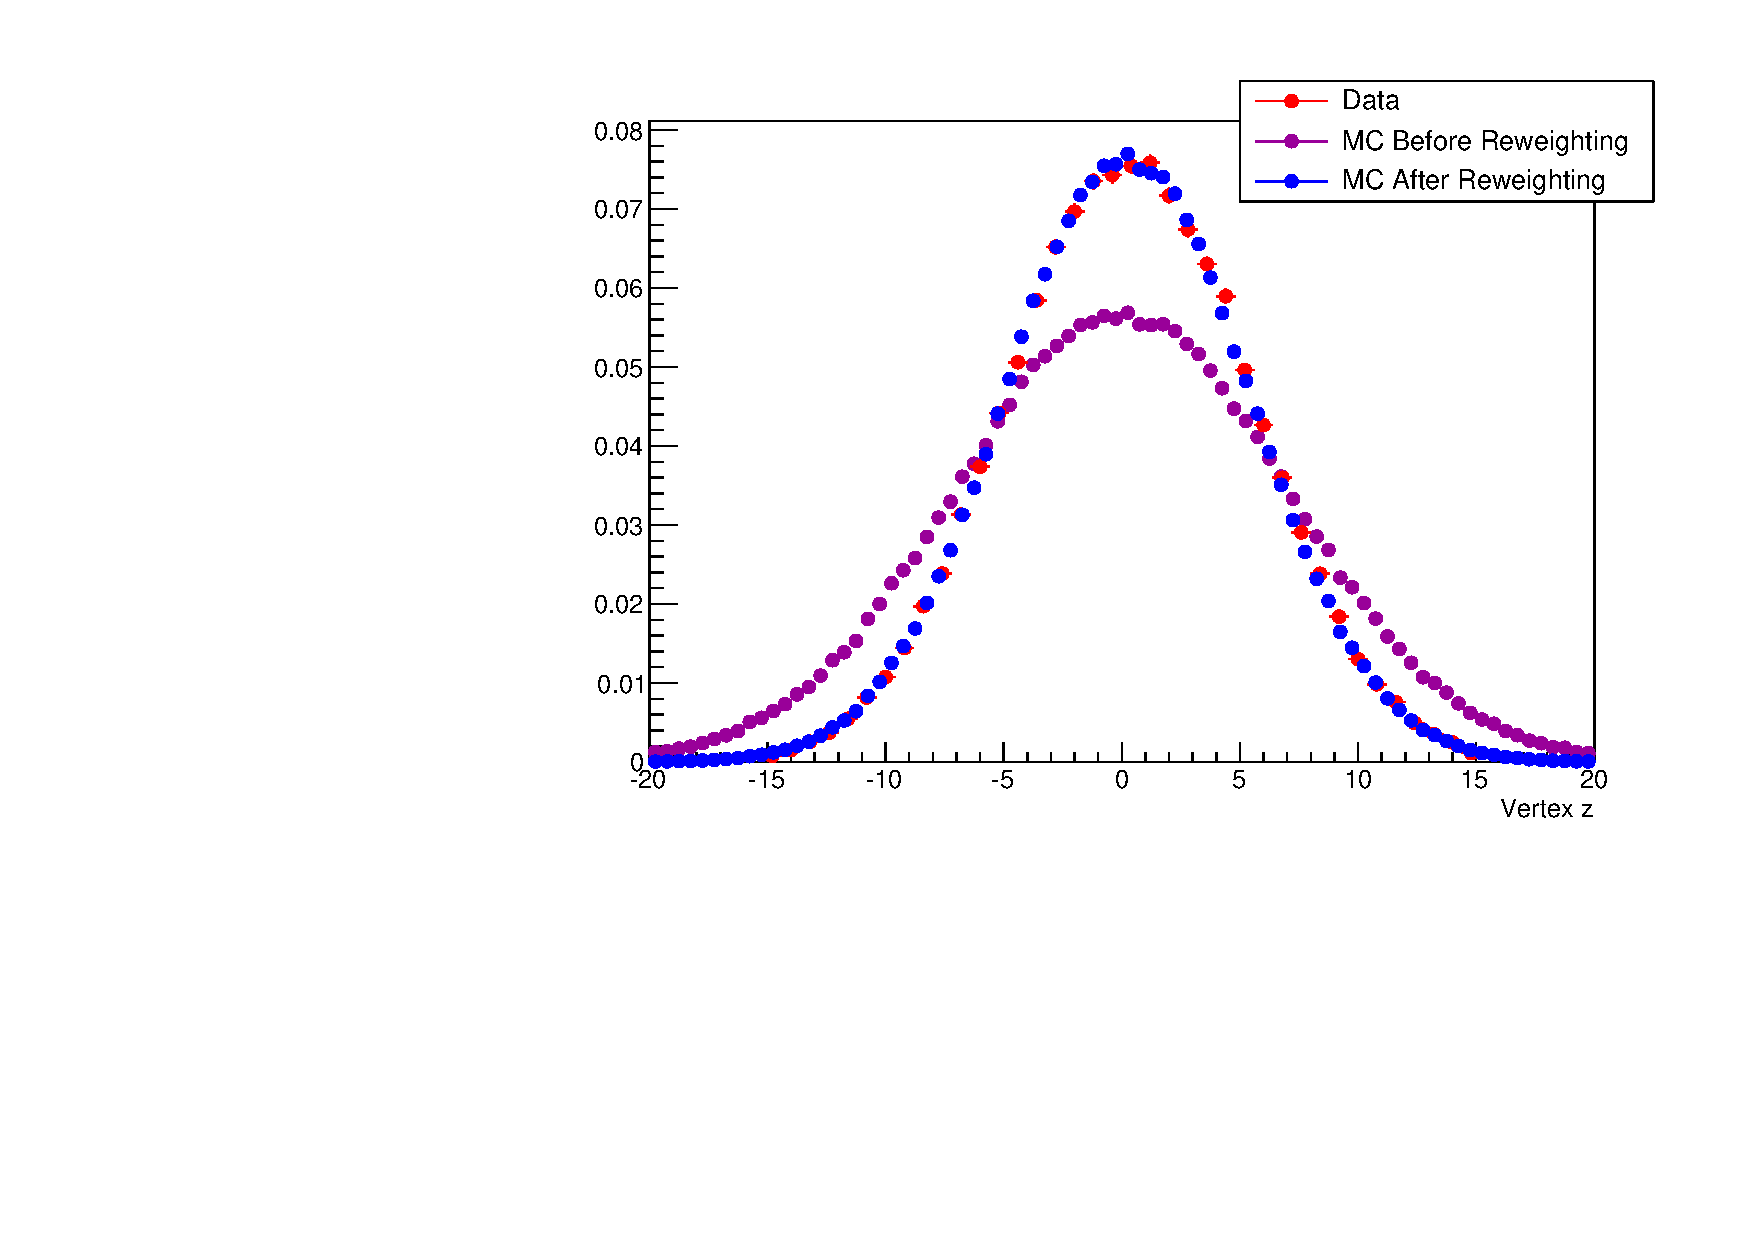
\includegraphics[width=0.58\linewidth]{figures/Samples/HydjetVzReweighting.pdf}
  \caption{
    Vertex z distribution for {\sc pythia+hydjet} reweighted to match centrality distribution of PbPb data.
  }
\label{fig:HydVz_Reweighting}
\end{center}
\end{figure}




\begin{figure}[ht]
\begin {center}
  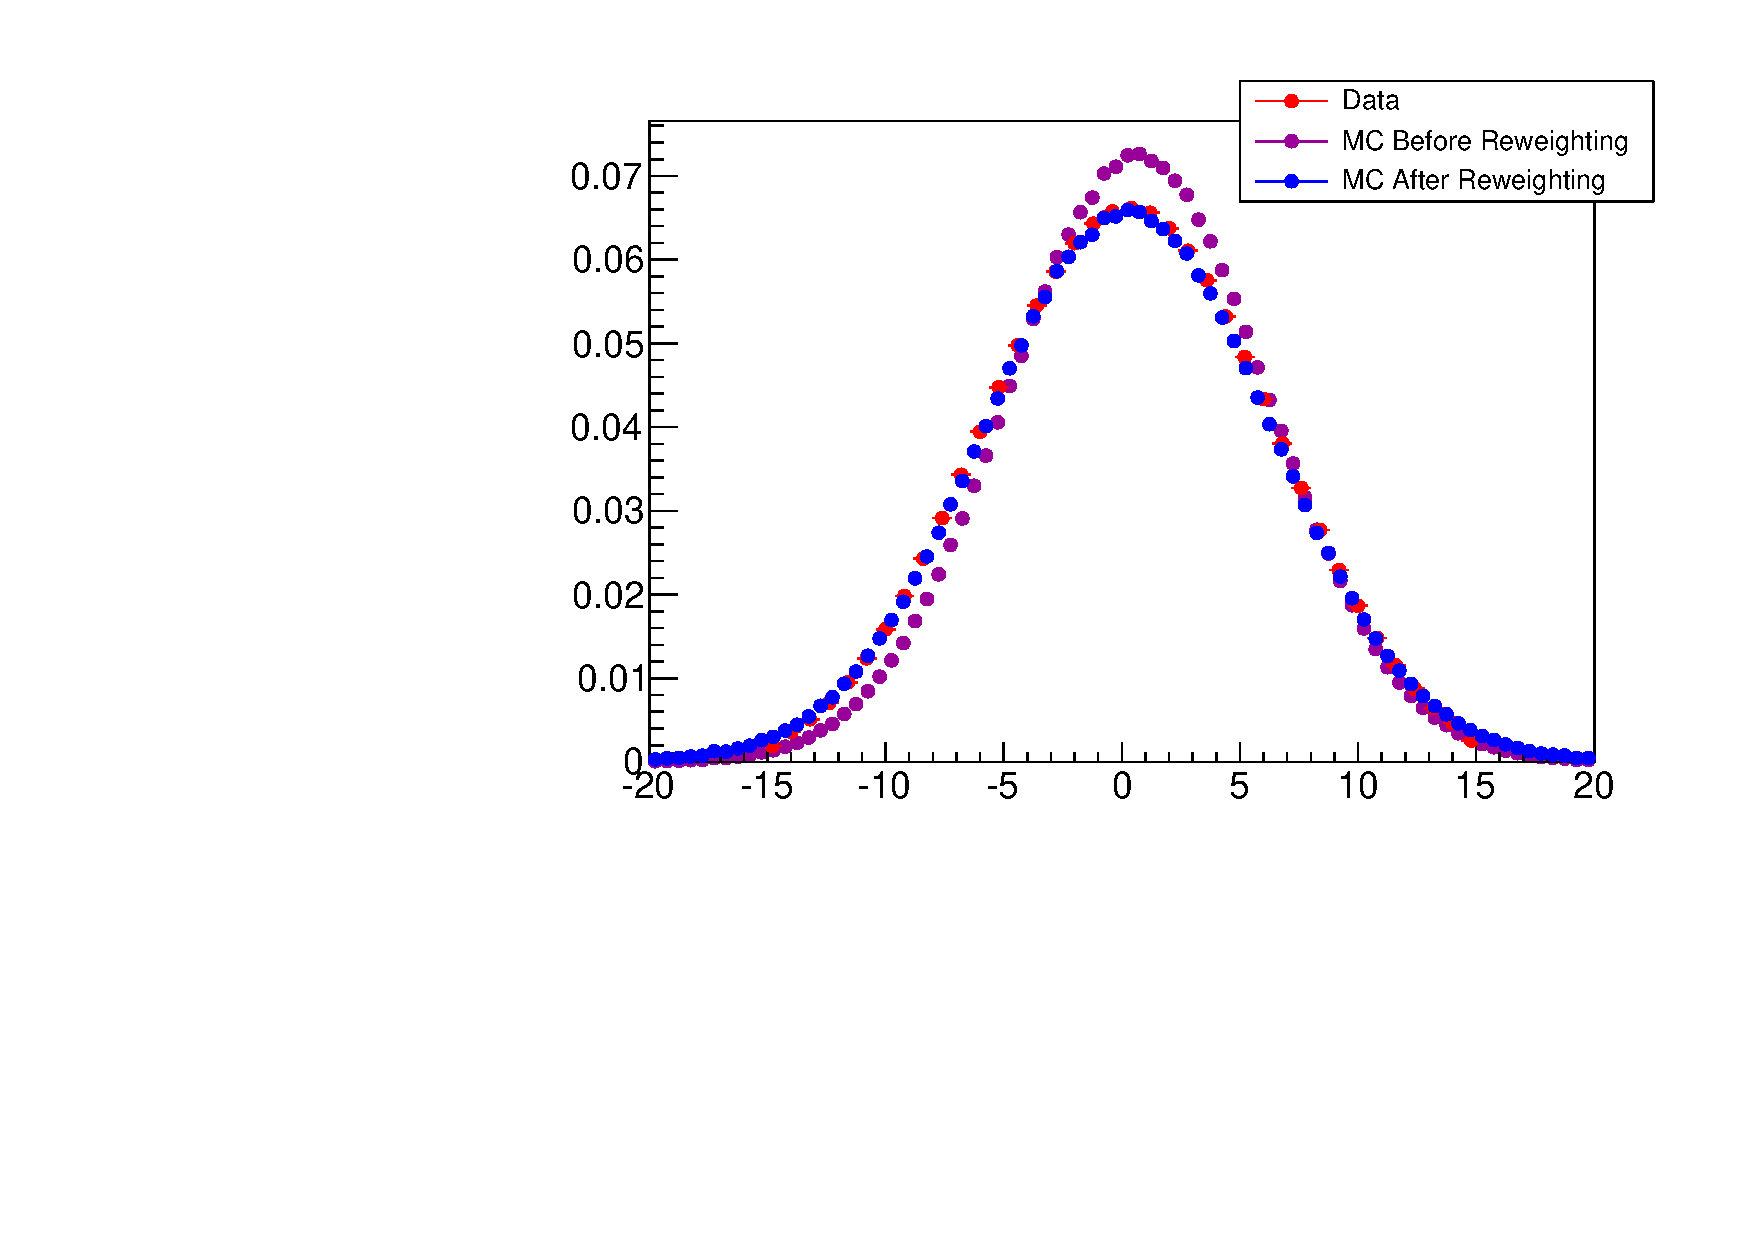
\includegraphics[width=0.58\linewidth]{figures/Samples/PythiaVzReweighting.pdf}
  \caption{
    Vertex z distribution for {\sc pythia} reweighted to match centrality distribution of pp data.
  }
\label{fig:PythiaVz_Reweighting}
\end{center}
\end{figure}


\subsubsection{Monte Carlo samples at 2.76 TeV}

Tables~\ref{mc_stats_276}  and~\ref{mc_stats_502} summarize the {\sc pythia} and {\sc pythia+hydjet} samples used in this analysis by $\hat{p_{\rm T}}$, with respective numbers of generated events and cross-sections used for combining samples. 

\begin{table}[htbp]
\begin{center} 
\caption{Summary of Monte Carlo samples and generated events at 2.76 TeV}

\label{mc_stats_276} \begin{tabular}{|c|c|c|c|}
\hline
Generator & Process & Cross section (mb) & Number of events \\
\hline
{\sc pythia+hydjet} & $\hat{p_{\rm T}}$ $> 50$~GeV & $1.025\times 10^{-3}$ & 395k  \\
{\sc pythia+hydjet} & $\hat{p_{\rm T}}$ $> 80$~GeV & $9.865\times 10^{-5}$ & 368k  \\
{\sc pythia+hydjet} & $\hat{p_{\rm T}}$ $> 120$~GeV & $1.129 \times 10^{-5}$ & 367k \\
{\sc pythia+hydjet} & $\hat{p_{\rm T}}$ $> 170$~GeV & $1.465 \times 10^{-6}$ & 392k \\
{\sc pythia+hydjet} & $\hat{p_{\rm T}}$ $> 220$~GeV & $2.837\times 10^{-7}$ & 181k \\
{\sc pythia+hydjet} & $\hat{p_{\rm T}}$ $> 280$~GeV & $2.837\times 10^{-7}$ & 50k \\
\hline
{\sc pythia} & $\hat{p_{\rm T}}$ $> 80$~GeV & $9.865\times 10^{-5}$ & 104k  \\
{\sc pythia} & $\hat{p_{\rm T}}$ $> 120$~GeV & $1.129 \times 10^{-5}$ & 975k \\
{\sc pythia} & $\hat{p_{\rm T}}$ $> 170$~GeV & $1.465 \times 10^{-6}$ & 69k \\

\hline
\end{tabular}
\end{center} 
\end{table} 


\clearpage

\subsubsection{Summary of Monte Carlo samples at 5.02 TeV}

\begin{table}[h!]
\begin{center} 
\caption{Summary of Monte Carlo samples and generated events at 5.02 TeV}

\label{mc_stats_502} \begin{tabular}{|c|c|c|c|}
\hline
\hline

Generator & Process & Cross section (mb) & Number of events \\
\hline
{\sc pythia+hydjet} & $\hat{p_{\rm T}}$ $> 80$~GeV/$c$ & $4.412\times 10^{-4}$ & 499k \\
{\sc pythia+hydjet} & $\hat{p_{\rm T}}$ $> 120$~GeV/$c$ & $ 6.147\times 10^{-5}$& 496k \\
{\sc pythia+hydjet} & $\hat{p_{\rm T}}$ $> 170$~GeV/$c$ &  $1.018\times 10^{-5}$ & 498k \\
{\sc pythia+hydjet} & $\hat{p_{\rm T}}$ $> 220$~GeV/$c$ &  $2.477\times 10^{-6}$ & 200k \\
{\sc pythia+hydjet} & $\hat{p_{\rm T}}$ $> 280$~GeV/$c$ &  $6.160\times 10^{-7}$ & 200k \\




\hline
{\sc pythia} & $\hat{p_{\rm T}}$ $> 80$~GeV/$c$ & $4.412\times 10^{-4}$ & 500k \\
{\sc pythia} & $\hat{p_{\rm T}}$ $> 120$~GeV/$c$ & $6.147\times 10^{-5}$& 500k \\
{\sc pythia} & $\hat{p_{\rm T}}$ $> 170$~GeV/$c$ & $1.018\times 10^{-5}$ & 499k \\
{\sc pythia} & $\hat{p_{\rm T}}$ $> 220$~GeV/$c$ & $2.477\times 10^{-6}$ & 200k \\
{\sc pythia} & $\hat{p_{\rm T}}$ $> 280$~GeV/$c$ & $6.160\times 10^{-7}$ & 200k \\


\hline
\hline

\end{tabular}
\end{center} 
\end{table} 


\clearpage


\subsection{Jet selection and dijet asymmetry classes}
\label{sec:jet_sel}

Jet selection in this analysis is restricted to the pseudorapidity region $|\eta_{\rm jet}| < 1.6$ to ensure stable reconstruction performance in the calorimeter barrel region.  A requirement is also imposed that the highest-$p_{\rm T}$ track contains no less than 1\% and no more than 98\% of the total jet $p_{\rm T}$.  In the jet selection refered to as ``inclusive jets'' for analysis at both 2.76 TeV and 5.02 TeV, all jets with $p_{\rm T, jet} > 120$~GeV are considered.  In this selection, it is possible to select more than one jet from the same event, provided that each jet satisfies the inclusive selection criteria. 

In addition to the inclusive jet selection, a ``dijet'' selection of events containing two back-to-back high-$p_{\rm T}$ jets is also analyzed for the 2.76 TeV data sample.  Events are included in this sample based on the criteria that they contain highest-$p_{\rm T}$ ``leading'' jet with $p_{\rm T,1} > 120$~GeV and a second-highest-$p_{\rm T}$ ``subleading'' jet with $p_{\rm T,2} > 50$~GeV with relative azimuthal separation $\Delta\phi > \frac{5\pi}{6}$.  This dijet sample is subdivided into a sample of relatively ``balanced'' dijets, with similar $p_{\rm T,1}$ and $p_{\rm T,2}$ and a sample of relatively ``unbalanced'' dijets in which the leading jet has a much larger $p_{\rm T}$ than the subleading jet based on asymmetry parameter $A_{\rm J}$. The balanced' selection is defined as those events for which $A_{\rm J} < 0.22$, while the unbalanced selection as defined as those events for which $A_{\rm J} > 0.22$.  The dividing value $A_{\rm J} = 0.22$ is chosen for consistency with previous CMS analyses~\cite{Chatrchyan:2011sx, HIN_2014_010}.  In this analysis, 52\% of central PbPb events are balanced, while 67\% of pp events are balanced.  Jet kinematics for all jet samples (broken down by asymmetry for 2.76 TeV dijet data) are shown in Appendix~\ref{app:kinematics_run1} for 2.76 TeV data and in Appendix~\ref{app:kinematics_run2} for 5.02 TeV data.

\subsection{Track selection and classes}

Tracks, reconstructed as described in Sec.~\ref{sec:Tracks} are required to satisfy the following criteria: 
\begin{itemize}
\item  $|\eta_{\rm trk}| < 2.4$ -- restricts to the barrel region of the tracker
\item  $0.5 < p_{\rm T}^{\rm trk} < 300$ GeV -- excludes very low-$p_{\rm T}$ tracks where reconstruction performance is not stable
\item High Purity criteria  -- see  Sec.~\ref{sec:high_purity}
\item Distance of closest approach (DCA) in x-y plane and in z less than 3 times the DCA error -- reduces fraction of tracks not associated with a primary vertex
\item Relative $p_{\rm T}^{\rm trk}$ error less than 30\% (10\% for 5.02 TeV PbPb data) -- removes tracks with very poor resolution (has a negligible effect on efficiency as CMS resolution is generally good) 
\end{itemize}

\noindent For 5.02 TeV PbPb data, the following additional criteria are also applied to reduce the contribution from misidentified tracks~\cite{AN-15-187}:
\begin{itemize}
\item Exclude tracks with fewer than 11 tracker hits
\item Require that for each track the chi-squared over number of degrees of freedom ($\chi^{2}$/ Ndof) of the track fit, also divided by the number of tracker layers (nLayer) hit as the track passed through the detector, is less than 0.15, i.e. $\chi^{2}$/Ndof/nLayer $< 0.15$.  
\item For tracks with $p_{\rm T} > 20$ GeV (the kinematic region in which misreconstruction is difficult to access with Monte Carlo), calorimeter matching is applied:  since high-$p_{\rm T}$ tracks eventually deposit their energy in a calorimeter after passing through the tracker, tracks are required to be associated with calorimeter transverse energy $E_{\rm T} = (E_{\rm ECAL} + E_{\rm HCAL})/\rm{cosh}(\eta_{\rm trk})$, such that $E_{\rm T} > 0.5 p_{\rm T}^{\rm trk}$ 

\end{itemize}

\noindent After these selection criteria are applied, tracking efficiency corrections are applied as described in Sec.~\ref{sec:track_eff}.  Tracks in this analysis are considered in the following classes:  0.5--1~GeV, 1--2~GeV, 2--3~GeV, 3--4~GeV, 4--8~GeV, 8--12~GeV, 12--16~GeV, 16--20~GeV, and above 20~GeV.   Not all bins are considered in every analysis, and for 5.02 TeV studies the lowest-$p_{\rm T}^{\rm trk}$ bin is 0.7--1~GeV.     

\clearpage

\subsection{Summary of analysis bins}

Table~\ref{table:bins} summarizes the key kinematic selections and bins for the three components to this analysis.  In all cases, identical selection is applied to PbPb and pp data.  Event, jet, and track quality cuts are not included in this table.

\begin{table}[h!]

\begin{center} 
\caption{Summary of data selections and analysis bins}
\label{table:bins} 
\begin{tabular}{|p{0.6in}|p{1.4in}|p{1.4in}|p{1.4in}|}
\hline
\hline
Variable & 2.76 TeV Inclusive & 5.02 TeV Inclusive & 2.76 TeV Dijets\\
\hline
PbPb & 0-10\%, 10-30\%,  & 0-10\%, 10-30\%, & 0-10\%, 10-30\%,\\
Centrality & 30-50\%, 50-100\% & 30-50\%, 50-100\% & 30-50\%, 50-100\%\\
\hline
Jet & $|\eta_{\rm jet}| < 1.6$ &  $|\eta_{\rm jet}| < 1.6$ &  $|\eta_{\rm jet}| < 1.6$ \\ 
Selection& $p_{\rm T} > $120~GeV & $p_{\rm T} > 120$~GeV & $p_{\rm T,1} > 120$~GeV\\
 &&&$p_{\rm T,2} > 50 $GeV\\
 &&&$\Delta\phi_{1,2}> \frac{5\pi}{6}$\\
 \hline
 $A_{\rm J}$ Bins & -- & -- &  $A_{\rm J} < 0.22$, \\
 &&&$A_{\rm J} > 0.22$\\
 \hline
 Track $\eta$ & $|\eta_{\rm trk}| < 2.4$ &$|\eta_{\rm trk}| < 2.4$ & $|\eta_{\rm trk}| < 2.4$ \\
 \hline
 $p_{\rm T}^{\rm trk}$ Bins & 1-2~GeV, 2-3~GeV, 3-4~GeV, 4-8~GeV & 0.7-1~GeV, 1-2~GeV, 2-3~GeV, 3-4~GeV, 4-8~GeV & 0.5-1~GeV, 1-2~GeV, 2-3~GeV, 3-4~GeV, 4-8~GeV, 8-300~GeV\\

\hline
\hline
\end{tabular}
\end{center} 
\end{table} 



